%%
%% This is file `sample-manuscript.tex',
%% generated with the docstrip utility.
%%
%% The original source files were:
%%
%% samples.dtx  (with options: `all,proceedings,bibtex,manuscript')
%%
%% IMPORTANT NOTICE:
%%
%% For the copyright see the source file.
%%
%% Any modified versions of this file must be renamed
%% with new filenames distinct from sample-manuscript.tex.
%%
%% For distribution of the original source see the terms
%% for copying and modification in the file samples.dtx.
%%
%% This generated file may be distributed as long as the
%% original source files, as listed above, are part of the
%% same distribution. (The sources need not necessarily be
%% in the same archive or directory.)
%%
%%
%% Commands for TeXCount
%TC:macro \cite [option:text,text]
%TC:macro \citep [option:text,text]
%TC:macro \citet [option:text,text]
%TC:envir table 0 1
%TC:envir table* 0 1
%TC:envir tabular [ignore] word
%TC:envir displaymath 0 word
%TC:envir math 0 word
%TC:envir comment 0 0
%%
%%
%% The first command in your LaTeX source must be the \documentclass
%% command.
%%
%% For submission and review of your manuscript please change the
%% command to \documentclass[manuscript, screen, review]{acmart}.
%%
%% When submitting camera ready or to TAPS, please change the command
%% to \documentclass[sigconf]{acmart} or whichever template is required
%% for your publication.
%%
%%
% \documentclass[manuscript,screen,review]{acmart}
\documentclass[acmsmall,sigconf]{acmart}

%%
%% \BibTeX command to typeset BibTeX logo in the docs
\AtBeginDocument{%
  \providecommand\BibTeX{{%
    Bib\TeX}}}

% %% Rights management information.  This information is sent to you
% %% when you complete the rights form.  These commands have SAMPLE
% %% values in them; it is your responsibility as an author to replace
% %% the commands and values with those provided to you when you
% %% complete the rights form.
% \setcopyright{acmlicensed}
% \copyrightyear{2018}
% \acmYear{2018}
% \acmDOI{XXXXXXX.XXXXXXX}

% %% These commands are for a PROCEEDINGS abstract or paper.
% \acmConference[Conference acronym 'XX]{Make sure to enter the correct
%   conference title from your rights confirmation emai}{June 03--05,
%   2018}{Woodstock, NY}
% %%
% %%  Uncomment \acmBooktitle if the title of the proceedings is different
% %%  from ``Proceedings of ...''!
% %%
% %%\acmBooktitle{Woodstock '18: ACM Symposium on Neural Gaze Detection,
% %%  June 03--05, 2018, Woodstock, NY}
% \acmISBN{978-1-4503-XXXX-X/18/06}


%%
%% Submission ID.
%% Use this when submitting an article to a sponsored event. You'll
%% receive a unique submission ID from the organizers
%% of the event, and this ID should be used as the parameter to this command.
%%\acmSubmissionID{123-A56-BU3}

%%
%% For managing citations, it is recommended to use bibliography
%% files in BibTeX format.
%%
%% You can then either use BibTeX with the ACM-Reference-Format style,
%% or BibLaTeX with the acmnumeric or acmauthoryear sytles, that include
%% support for advanced citation of software artefact from the
%% biblatex-software package, also separately available on CTAN.
%%
%% Look at the sample-*-biblatex.tex files for templates showcasing
%% the biblatex styles.
%%

%%
%% The majority of ACM publications use numbered citations and
%% references.  The command \citestyle{authoryear} switches to the
%% "author year" style.
%%
%% If you are preparing content for an event
%% sponsored by ACM SIGGRAPH, you must use the "author year" style of
%% citations and references.
%% Uncommenting
%% the next command will enable that style.
%%\citestyle{acmauthoryear}

\usepackage{mathtools}

\graphicspath{{images/}}
\DeclareGraphicsExtensions{.pdf}

\DeclarePairedDelimiter{\set}{\{}{\}}
\DeclarePairedDelimiter{\tuple}{(}{)}
\DeclarePairedDelimiter{\abs}{\lvert}{\rvert}
\renewcommand{\implies}{\rightarrow}
\newcommand{\db}{\mathcal{D}}
\newcommand{\model}{\mathcal{M}}
\newcommand{\priv}{R}
\newcommand{\pos}{\hat{P}}
\newcommand{\posm}{\hat{P}_\mathcal{M}}
\newcommand{\tru}{T}
\newcommand{\leg}{L}
\newcommand{\sco}{\hat{S}}
\newcommand{\scom}{\hat{S}_\mathcal{M}}
\newcommand{\calib}{C}
\newcommand{\prob}[1]{\text{Pr}[#1]}

%%
%% end of the preamble, start of the body of the document source.
\begin{document}

%%
%% The "title" command has an optional parameter,
%% allowing the author to define a "short title" to be used in page headers.
\title{The Name of the Title Is Hope}

%%
%% The "author" command and its associated commands are used to define
%% the authors and their affiliations.
%% Of note is the shared affiliation of the first two authors, and the
%% "authornote" and "authornotemark" commands
%% used to denote shared contribution to the research.
\author{Chih-Cheng Rex Yuan}
\email{hello@rexyuan.com}
\affiliation{%
  \institution{Institute of Information Science, Academia Sinica}
  \city{Taipei}
  \country{Taiwan}
}

\author{Bow-Yaw Wang}
\email{bywang@iis.sinica.edu.tw}
\affiliation{%
  \institution{Institute of Information Science, Academia Sinica}
  \city{Taipei}
  \country{Taiwan}
}

%%
%% By default, the full list of authors will be used in the page
%% headers. Often, this list is too long, and will overlap
%% other information printed in the page headers. This command allows
%% the author to define a more concise list
%% of authors' names for this purpose.
% \renewcommand{\shortauthors}{Trovato et al.}

%%
%% The abstract is a short summary of the work to be presented in the
%% article.
\begin{abstract}
  abstract
\end{abstract}

% %%
% %% The code below is generated by the tool at http://dl.acm.org/ccs.cfm.
% %% Please copy and paste the code instead of the example below.
% %%
% \begin{CCSXML}
% <ccs2012>
%  <concept>
%   <concept_id>00000000.0000000.0000000</concept_id>
%   <concept_desc>Do Not Use This Code, Generate the Correct Terms for Your Paper</concept_desc>
%   <concept_significance>500</concept_significance>
%  </concept>
%  <concept>
%   <concept_id>00000000.00000000.00000000</concept_id>
%   <concept_desc>Do Not Use This Code, Generate the Correct Terms for Your Paper</concept_desc>
%   <concept_significance>300</concept_significance>
%  </concept>
%  <concept>
%   <concept_id>00000000.00000000.00000000</concept_id>
%   <concept_desc>Do Not Use This Code, Generate the Correct Terms for Your Paper</concept_desc>
%   <concept_significance>100</concept_significance>
%  </concept>
%  <concept>
%   <concept_id>00000000.00000000.00000000</concept_id>
%   <concept_desc>Do Not Use This Code, Generate the Correct Terms for Your Paper</concept_desc>
%   <concept_significance>100</concept_significance>
%  </concept>
% </ccs2012>
% \end{CCSXML}

% \ccsdesc[500]{Do Not Use This Code~Generate the Correct Terms for Your Paper}
% \ccsdesc[300]{Do Not Use This Code~Generate the Correct Terms for Your Paper}
% \ccsdesc{Do Not Use This Code~Generate the Correct Terms for Your Paper}
% \ccsdesc[100]{Do Not Use This Code~Generate the Correct Terms for Your Paper}

% %%
% %% Keywords. The author(s) should pick words that accurately describe
% %% the work being presented. Separate the keywords with commas.
% \keywords{Do, Not, Us, This, Code, Put, the, Correct, Terms, for,
%   Your, Paper}

\received{20 February 2007}
\received[revised]{12 March 2009}
\received[accepted]{5 June 2009}

%%
%% This command processes the author and affiliation and title
%% information and builds the first part of the formatted document.
\maketitle

\section{Introduction}

\section{Related Work}

\section{Auditing Framework}

\subsection{Preliminaries}

A \emph{row} $r_i$ is a lookup table or dictionary. A \emph{database} $\db = \set{r_1, r_2, ...}$ is a collection of rows. The attributes of $\db$ is $\mathcal{A} = \set{A_1, A_2, ...}$. The domain of $A_i$ is $\Omega_i$.

Let $C \subseteq \mathcal{A}$. Let $\Omega_C = \Pi_{i \in C} \Omega_i$. The \emph{marginal}\cite{barak2007privacy,mckenna2021winning} on $C$ is a vector $\mu \in \mathbb{R}^{\abs{\Omega_C}}$, indexed by domain element $t \in \Omega_C$, such that each entry is a count $\mu_t = \Sigma_{x \in \db} \vmathbb{1} [x_C = t]$ where $\vmathbb{1}$ is the indicator function. Let $M_C(\db)$ be the function that computes the marginal on $C$, i.e., $\mu = M_C(\db)$.

A \emph{randomized mechanism} is a randomized algorithm $M$ that takes a database $\db$ and, after, introducing noise, outputs some results in set $R$.

The $p$-norm is denoted by $L_p$ and the $p$-norm of a vector $x$ is denoted by $\Vert x \Vert_p$.

The normal distribution or Gaussian distribution with mean $\mu$ and standard deviation $\sigma$ is denoted by $\mathcal{N}(\mu, \sigma^2)$.

The Kullback–Leibler divergence between probability distributions $P$ and $Q$ is denoted by $D_{KL}(P \Vert Q)$. The generalization of it, R\'enyi divergence\cite{van2014renyi}, of order $\alpha$ is denoted by $D_\alpha(P \Vert Q)$.

\subsection{Fairness Measures}

\subsection{Differential Privacy}

\begin{definition}[Sensitivity\cite{dwork2014algorithmic}]\label{def:sensitivity}
Let $f$ be a function that takes a database $\db$ and outputs a vector $\mathbb{R}^p$. The $L_2$ sensitivity of $f$ is for all databases $\db_1,\db_2$ that differ in exactly one row:
\[
\Delta^2_f = max_{\db_1,\db_2} \Vert f(\db_1) - f(\db_2) \Vert_p
\]
\end{definition}

\begin{definition}[Gaussian Mechanism\cite{dwork2014algorithmic}]\label{def:gm}
Let $f$ be a function that takes a database $\db$ and outputs a vector $\mathbb{R}^p$. The Gaussian Mechanism $M$ adds Gaussian noise with scale $\sigma$ to each of the $p$ outputs:
\[
M(\db) = f(\db) + \mathcal{N}(0, \sigma^2 \mathbb{I})
\]
\end{definition}

\begin{definition}[Differential Privacy (DP) \cite{dwork2006calibrating,dwork2014algorithmic,mckenna2021winning}]\label{def:rdp}
A randomized mechanism $M$ satisfies $(\epsilon,\delta)$-DP if, for all databases $\db_1,\db_2$ that differ in exactly one row and for all subsets $S$ of $R$, we have
\[
\prob{M(\db_1) \in S} \leq e^\epsilon \prob{M(\db_2) \in S} + \delta
\]
\end{definition}

\begin{definition}[R\'enyi Differential Privacy (RDP)]\label{def:rdp}
A randomized mechanism $M$ satisfies $(\alpha,\gamma)$-RDP for $\alpha \geq 1$ and $\gamma \geq 1$ if, for all databases $\db_1,\db_2$ that differ in exactly one row, we have
\[
D_\alpha(M(\db_1) \Vert M(\db_2)) \leq \gamma
\]
\end{definition}

\begin{theorem}[RDP of the Gaussian Mechanism\cite{feldman2018privacy,mironov2017renyi}]
The Gaussian Mechanism satisfies $(\alpha, \alpha \frac{\Delta^2_f}{2 \sigma^2})$-RDP.
\end{theorem}

\subsection{Synthetic Data}

\section{Methodology}

\subsection{Differential Private Synthetic Data}

\subsection{Fairness Checker}

\subsection{Implementation}

\section{Results}

\subsection{Adult Income Dataset}

\subsection{COMPAS Dataset}

\subsection{One More Dataset}

\section{Discussion}

\subsection{Accuracy}

\subsection{Impossibility}

\section{Conclusion}

Some examples.  A paginated journal article \cite{Abril07}

% \begin{table}
%   \caption{Frequency of Special Characters}
%   \label{tab:freq}
%   \begin{tabular}{ccl}
%     \toprule
%     Non-English or Math&Frequency&Comments\\
%     \midrule
%     \O & 1 in 1,000& For Swedish names\\
%     $\pi$ & 1 in 5& Common in math\\
%     \$ & 4 in 5 & Used in business\\
%     $\Psi^2_1$ & 1 in 40,000& Unexplained usage\\
%   \bottomrule
% \end{tabular}
% \end{table}

% \begin{table*}
%   \caption{Some Typical Commands}
%   \label{tab:commands}
%   \begin{tabular}{ccl}
%     \toprule
%     Command &A Number & Comments\\
%     \midrule
%     \texttt{{\char'134}author} & 100& Author \\
%     \texttt{{\char'134}table}& 300 & For tables\\
%     \texttt{{\char'134}table*}& 400& For wider tables\\
%     \bottomrule
%   \end{tabular}
% \end{table*}

\begin{figure}[h]
  \centering
  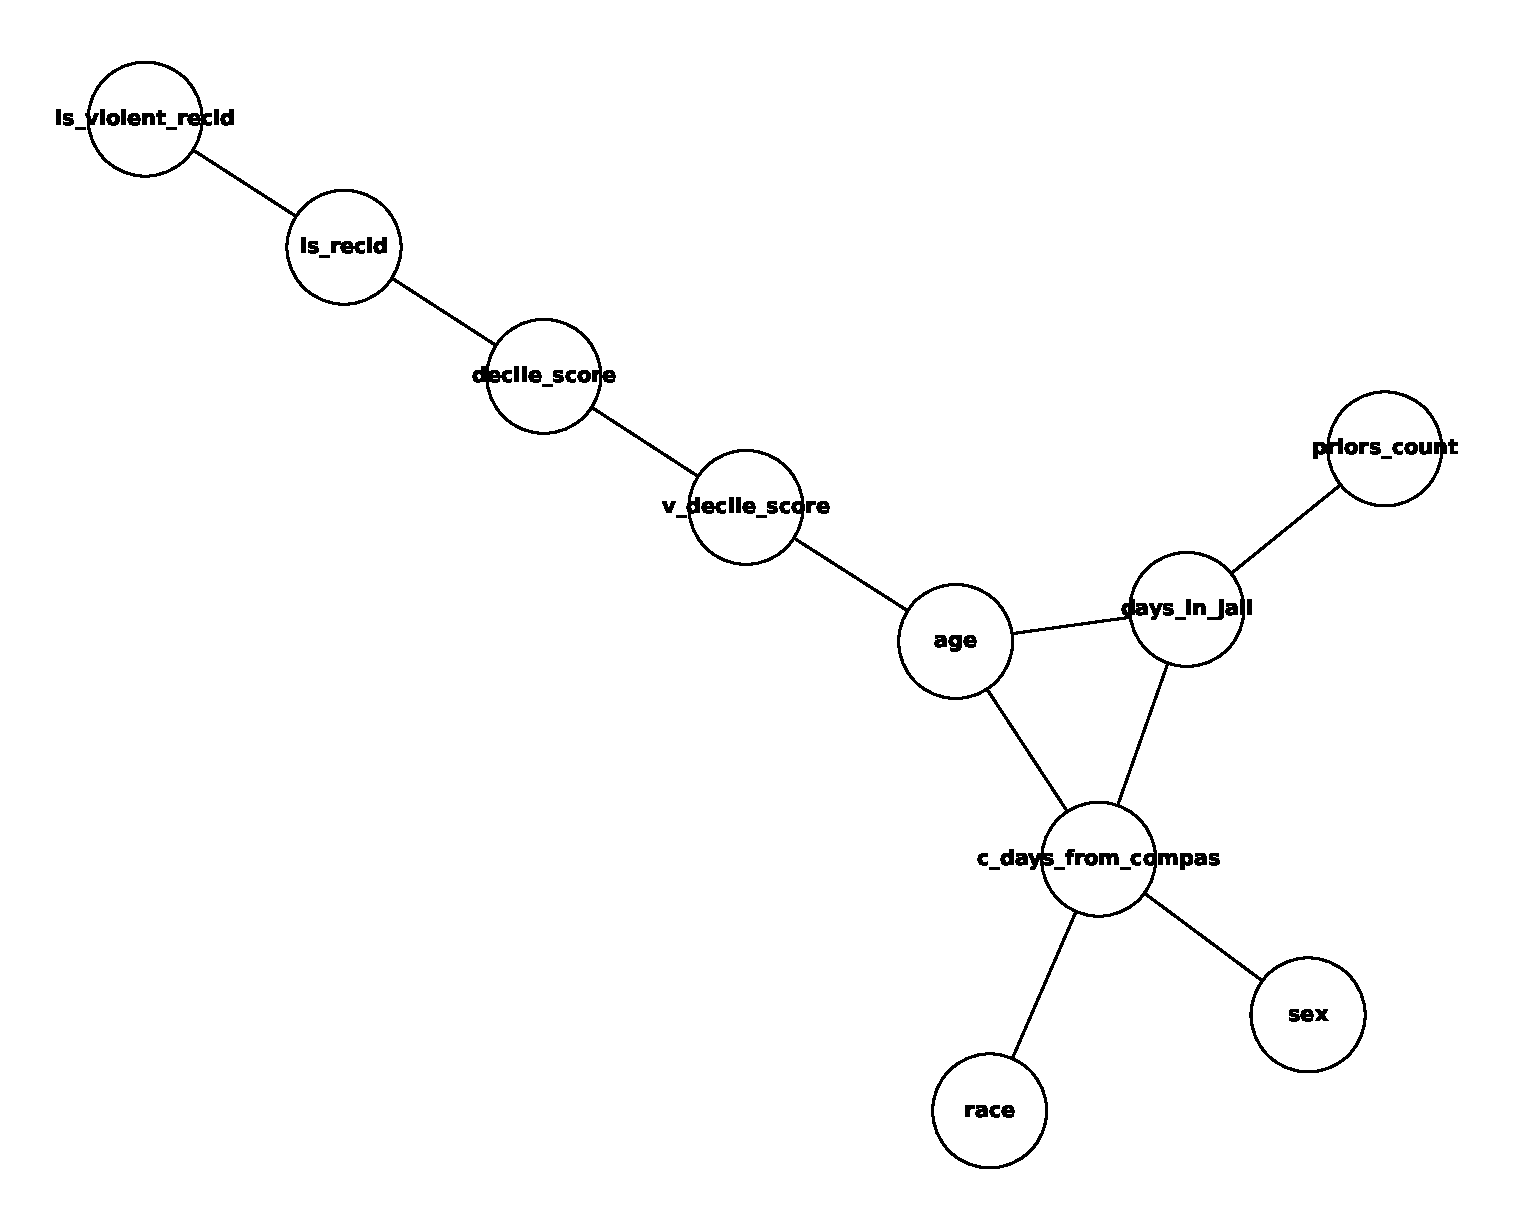
\includegraphics[width=\linewidth]{compas_mst}
  \caption{1907 Franklin Model D roadster. Photograph by Harris \&
    Ewing, Inc. [Public domain], via Wikimedia
    Commons. (\url{https://goo.gl/VLCRBB}).}
  \Description{A woman and a girl in white dresses sit in an open car.}
\end{figure}

\begin{figure}[h]
  \centering
  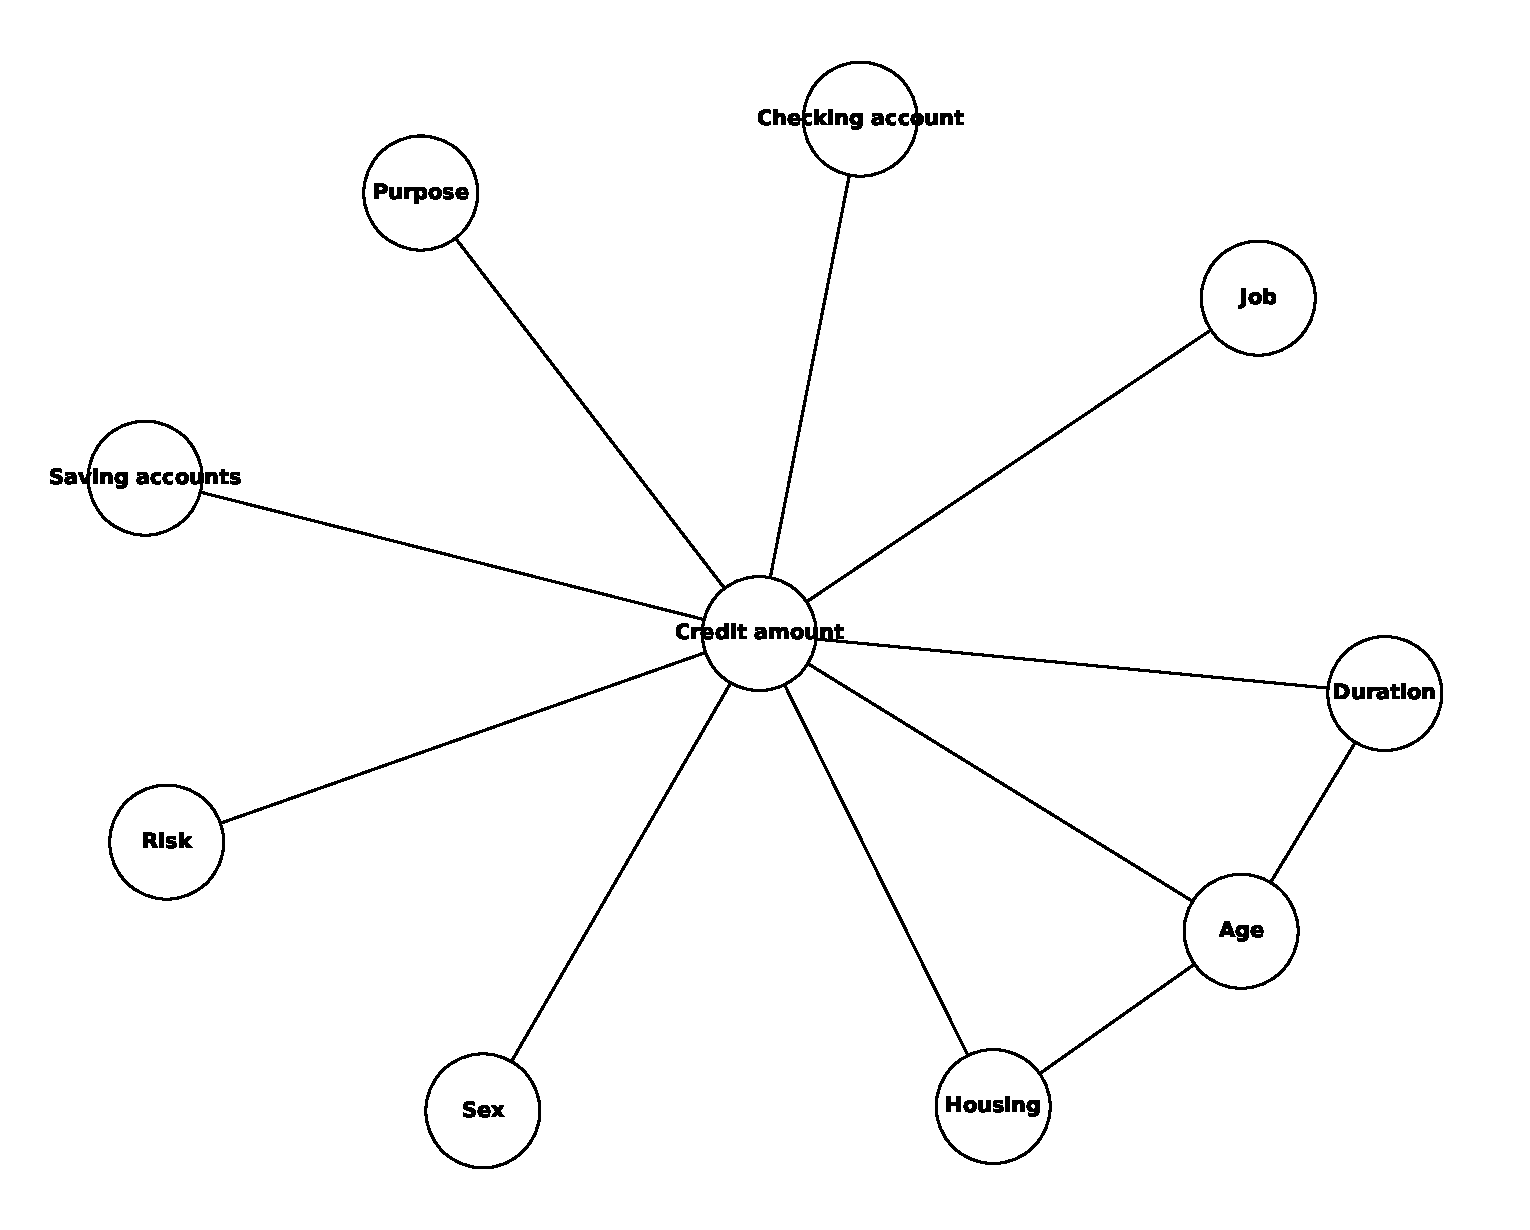
\includegraphics[width=\linewidth]{adult_mst}
  \caption{1907 Franklin Model D roadster. Photograph by Harris \&
    Ewing, Inc. [Public domain], via Wikimedia
    Commons. (\url{https://goo.gl/VLCRBB}).}
  \Description{A woman and a girl in white dresses sit in an open car.}
\end{figure}

%%
%% The acknowledgments section is defined using the "acks" environment
%% (and NOT an unnumbered section). This ensures the proper
%% identification of the section in the article metadata, and the
%% consistent spelling of the heading.
% \begin{acks}
% To Robert, for the bagels and explaining CMYK and color spaces.
% \end{acks}

%%
%% The next two lines define the bibliography style to be used, and
%% the bibliography file.
\bibliographystyle{ACM-Reference-Format}
\bibliography{references}


%%
%% If your work has an appendix, this is the place to put it.
% \appendix

\end{document}
\endinput
%%
%% End of file `sample-manuscript.tex'.
